\documentclass{article}


\usepackage{amsmath}

\DeclareMathOperator*{\argmin}{arg\,min} %argmin

\usepackage{floatrow}
% Table float box with bottom caption, box width adjusted to content
\newfloatcommand{capbtabbox}{table}[][\FBwidth]
\usepackage{caption}
\usepackage{subcaption}
\captionsetup{compatibility=false}

%%%

\usepackage{array}
% For tabulars
\newcolumntype{P}[1]{>{\centering\arraybackslash}p{#1}}

\usepackage{pdfpages}
\usepackage{graphicx}
\usepackage{longtable}
%\usepackage[export]{adjustbox}
%\usepackage{tabu}
\usepackage{xcolor,colortbl}
\usepackage{caption}
\usepackage{subcaption}
\usepackage{float}
\usepackage{wrapfig}
\usepackage{amsfonts}
\usepackage{amsthm}

\usepackage[margin=0.65in]{geometry}
\usepackage{url} % for bibliograpy links
\begin{document}

\vspace*{3ex}
\begin{flushright}
{\large 10 November 2015}
\end{flushright}

\vskip20ex
\hskip3cm

\begin{center}


\begin{figure}[H]
\centering
\begin{subfigure}{.5\textwidth}
  \centering
  
\includegraphics[width=.9\linewidth]{images/mini.png}
\end{subfigure}%
\begin{subfigure}{.5\textwidth}
  \centering
  
\includegraphics[width=.9\linewidth]{images/pw.jpg}
\end{subfigure}
\end{figure}




\Large {\bf
	Bachelor Thesis \\
	Finite Automata for Pattern Recognition
}

\Large {\bf 
	Technical Project
}
\end{center}
\vskip2ex


\vskip25ex

\begin{flushleft}
{\large Bartlomiej Dybisz \\
Jakub Ciecierski

}
\end{flushleft}

\newpage
\tableofcontents
\newpage

%------------------------------------------------------------------------------

\section*{Document metric}

\begin{center}


\begin{table}[h]
\hspace*{-1.1cm}
\large
\begin{tabular}{|
>{\columncolor[HTML]{C0C0C0}}l |l|l|l|l|l|}
\hline
\multicolumn{6}{|l|}{\cellcolor[HTML]{C0C0C0}Document metric}                                                                                                                                         \\ \hline
Project:       & \multicolumn{2}{l|}{Finite automata for pattern recognition} & 
\cellcolor[HTML]{C0C0C0}Company: & \multicolumn{2}{l|}{WUT}                                               \\ \hline
Name:          & \multicolumn{5}{l|}{Technical Project}                                                                                                                                       \\ \hline
Topics:        & \multicolumn{5}{l|}{Architecture and algorithms defining the project}                                                                                                                                       \\ \hline
Author:        & \multicolumn{5}{l|}{Jakub Ciecierski, Bartlomiej Dybisz}                                                                                                                                                \\ \hline
File:          & \multicolumn{5}{l|}{technical\_project.pdf}                                                                                                                                      \\ \hline
Version no:    & 0.1                                                                      & \cellcolor[HTML]{C0C0C0}Status:  & Under development & \cellcolor[HTML]{C0C0C0}Opening date: & 2015-10-27 \\ \hline
Summary:       & \multicolumn{5}{l|}{Technical side of research on pattern recognition by finite automata}                                                                                                           \\ \hline
Authorized by: & \begin{tabular}[c]{@{}l@{}}Wladyslaw Homenda\end{tabular} & \multicolumn{3}{l|}{\cellcolor[HTML]{C0C0C0}Last modification date:}                         & 2015-11-10 \\ \hline
\end{tabular}
\end{table}

\end{center}



\section*{History of changes}

\begin{center}


\begin{table}[h]
\hspace*{-1.0cm}
\large
\begin{tabular}{|l|l|l|l|}
\hline
\multicolumn{4}{|l|}{\cellcolor[HTML]{C0C0C0}History of Changes} \\ \hline
Version         & Date         & Who        & Description        \\ \hline

0.1         
& 2015-11-10
& Jakub Ciecierski, Bartlomiej Dybisz
& Definition of the main purpose of the document       \\ \hline
\end{tabular}
\end{table}

\end{center}


%---------------------------------------------------------------

\section*{Schedule}

\begin{center}


\begin{table}[h]

\large
\begin{tabular}{|l|l|l|}
\hline
\multicolumn{3}{|l|}{\cellcolor[HTML]{C0C0C0}Schedule} \\ \hline
Date         & Note        & Planned Progress          \\ \hline
\hline

27.10.2015   & Lab1    & Presentation of Business Analysis   \\ \hline
03.11.2015   &    & Additional changes of Business Analysis   \\ \hline
7-9.11.2015   &     & First drafts of UML of particular modules   \\ \hline
14-16.11.2015   &     & Requirements analysis, design of algorithms and further UML development \\ \hline
17.11.2015   &  Lab2   & Presentation of Technical Analysis   \\ \hline
20-22.11.2015   &     & Implementation of mudules needed for testing and basic GUI   \\ \hline
30.11.2015   & Lab3    & Presentation of results of tests on synthetic and semi-synthetic data  \\ \hline
4-6.12.2015   &     & GUI and console application development  \\ \hline
15.12.2015   & Lab4    & Final GUI  \\ \hline
-------  & -------    & Work depends on acquired results  \\ \hline
08.01.2015  & Lab5    & Complete system presentation  \\ \hline
\end{tabular}
\end{table}

\end{center}


%---------------------------------------------------------------
\newpage




%---------------------------------------------------------------
\section{Production Model}
{\bf Waterfall} model is a model which was developed for software development; that is to create software. It is called as such because the model develops systematically from one phase to other in a downward fashion, like a waterfall.


\begin{center}

	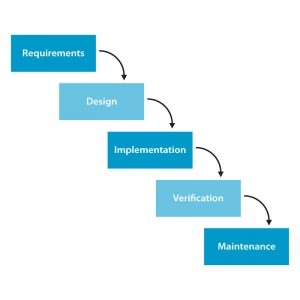
\includegraphics[width=80mm]{images/waterfall_model.jpg}

\end{center}


%---------------------------------------------------------------
\section{Technology}

%---------------------------------------------------------------
%---------------------------------------------------------------
\subsection{Algorithm Implementation}

The technology chosen to develop the implementation needed in the research is c++11 running under Linux OS. The c++ language allows to carefully control the computations by easily manipulating with the data. It is also been proven that c++ is one of the most efficient programming languages. The c++11 version of the language provides many modern features like smart pointers, lambda expression and new containers. Finally, the convenience of Makefile usage motivates us to work under Linux OS. The entire project can be built by a single command in the Makefile.

The implementation will be tested using unit test library called Google Test which is based on xUnit architecture. It supports automatic test discovery, a rich set of assertions and above all it is very clean and easy to use.


%---- JC ----%


%---- BD ----%
\subsection{Graphical User Interface}

To create Graphical User Interface, we will use JavaFx technology. It is a set of graphics and media packages that enables developers to design, create, test, debug, and deploy rich client applications that operate consistently across diverse platforms. Written as a Java API, JavaFX application code can reference APIs from any Java library. For example, JavaFX applications can use Java API libraries to access native system capabilities and connect to server-based middleware applications \cite{javafx_description}. Since GUI will be simple and straight forward, this technology will provide cross-platform character of the application and help us develop it in no time. Only basic user interface elements such as buttons, text fields, label etc will be used, hence we do not demand any sophisticated API.


%---------------------------------------------------------------
\section{Introduction}
Pattern Recognition focuses on building machines that can recognize pattern in various fields such as speech, fingerprint or optical characters. A pattern can be defined as feature vector and a label. Label informs us to which class a given element belongs to.

Assume that

To start with, in section~\ref{sec:prelim} preliminaries mathematical knowledge is presented. In section~\ref{sec:algorithms} the first sketch of algorithms defining the classifier is presented.

Finally, the architecture side of the project is introduced in section~\ref{sec:model}.


%---------------------------------------------------------------------
\section{Preliminaries}\label{sec:prelim}

%---------------------------------------------------------------------
%---------------------------------------------------------------------
\subsection{Hamming Distance} \label{sec:hamming}

%\begin{definition}
Hamming distance $H_d$ between two string of the same length is the number of positions at which the corresponding symbols differ.
%\end{definition}

%\begin{example} 
Let $w = John$ and $v = Jhon$. Notice that the symbols at positions two and three differ. Thus the Hamming distance between these two strings is $H_d(w,v) = 2$.
%\end{example}

%---------------------------------------------------------------------
%---------------------------------------------------------------------
\subsection{Cluster Evaluation} \label{sec::cluster}

Clustering is a method of segregating elements of a given data set into groups. Elements similar to each other should fall into one group while dissimilar elements are supposed to be separated.

The problem arises when no prior information about the structure of the data is given. At that point we can not simply assume number of clusters for the partitioning. The methods that estimate the optimal number of clusters in the given data set are now presented.

%---------------------------------------------------------------------
%---------------------------------------------------------------------
%---------------------------------------------------------------------
\subsubsection{K-Means}

K-means algorithm is a tool for clustering a given data set.
The goal of that algorithm is to partition a data set $X$ of size $n$ into $k$ clusters, where each $x_{j}\in X$ is assigned a single cluster. In order to do that, we find cluster centroids $\mu_{i}, i=1,\ldots,k$ that minimize the distance from the elements from data set. Formally k-means solves the following optimization problem:
\begin{equation}
  \argmin_{C}\sum_{i=1}^{k}\sum_{x\in C_{i}} d(x,\mu_{i})
\end{equation}
where $C_{i}$ is the set of elements that correspond to $i$-th cluster and $d(x,\mu_{i})$ is a~chosen distance measure between element $x$ and the cluster center $\mu_{i}$. At the first stage of the algorithm k centroids $\mu_{i}$ are selected. Then each element is assigned to the closest cluster. The centroids are updated with the mean of all points belonging to the corresponding cluster
\begin{equation}
  \mu_{i} = \frac{1}{|C_{i}|} \sum_{x\in C_{i}} x
\end{equation}

This process is repeated until convergence. It is worth mentioning that k-means might not find the best possible 
configuration.

The following summarises the k-means algorithm:

\begin{center}


\begin{enumerate}
	\item 
		Select $k$ initial centroids
	\item \label{enum:km_grp} 
		Group points to their closest centroids.
	\item \label{enum:km_centroids} 
		Update centroids by computing center of gravity - mean
	\item 
		Repeat~\ref{enum:km_grp} and~\ref{enum:km_centroids} until convergence or after maximum iterations.
\end{enumerate}

\end{center}

The method of choosing initial centroids can have a big impact on the result and the complexity. The naive method of initialization would involve using uniform distribution to randomly select k centroids among the data set. Such approach can easily define two centroids within a single potential cluster and thus k-means can get stuck in local optimum.
The k-means++ (k-means plus plus), algorithm proposes a better solution for initialization by spreading out the centroids. At the beginning, the first centroid is chosen as usual uniformly from the data set. Then for each data point $x$ we compute $D(x)$ which defines the distance between $x$ and the nearest centroid that have already been chosen. The next centroids is chosen by selecting a point from data set using weighted probability distribution proportional to $D(x)^2$. The process is repeated until all $k$ centroids are found.

The formal flow of the algorithm is now presented:

\begin{enumerate}
	\item 
		Choose the first centroid uniformly from data set.
	\item \label{enum:kmpp_dx}
		For $x$ in data set:
		\begin{enumerate}
			\item
				Compute $D(x)$, the distance between x and its nearest centroid.
		\end{enumerate}
		
	\item \label{enum:kmpp_weight}
		Select next centroid from data set with probability:
		$\frac{D(x)^2}{\sum_{x}D(x)^2}$
	\item 
		Repeat steps~\ref{enum:kmpp_dx} and~\ref{enum:kmpp_weight} until $k$ centroids are found.
\end{enumerate}

%---------------------------------------------------------------------
%---------------------------------------------------------------------
%---------------------------------------------------------------------
\subsubsection{McClain-Rao}
The McClain-Rao algorithm tries to select the optimal number of clusters for given data set. Let's define few measures needed to compute McClain-Rao index. Firstly we define the sum within-cluster distances $S_w$. It sums up all the distances of any two points from the same cluster. Formally $S_w$ is defined by the equation: 
\begin{equation}
	S_w = \sum_{l=0}^{k} \sum_{i < j \in I_l} d(x_i, x_j)
\end{equation}
where $I_l$ is the set of indices of the $l$-th cluster. Let $N_w$ be the total number of distances between pairs of points belonging to the same cluster.

Further, the sum of between-cluster distances $S_b$ is the sum of distances of points belonging to different clusters. The following equations describes it:
\begin{equation}
	S_b = \sum_{l < l^{'}}^{k} \sum_{i \in I_{l}, j \in I_{l^{'}}}  d(x_i, x_j)
\end{equation}
Similarly, let $N_b$ be the total number of distances between pairs of points which do not belong to the same cluster.

Finally, The McClain-Rao index $C$ is defined by equation: 
\begin{equation}
	C =  (\frac{S_w}{N_w}) / (\frac{S_b}{N_b})
\end{equation}

$C$ is the quotient between the mean within-cluster and between-cluster distances.
Note that the smaller the value of $C$ the better the clustering.

%---------------------------------------------------------------------
%---------------------------------------------------------------------
\subsection{Automaton} \label{sec:autom}
%\begin{definition}
Automaton is a system of five fields:
\begin{center}
	$A = (Q, \Sigma, \delta, q_0, F)$
\end{center}

where \\
$Q$ - finite set of states. \\
$\Sigma$ - Finite input alphabet. \\
$\delta$ - transition function. $\delta: Q \times \Sigma \rightarrow Q$ \\
$q_0$ - the initial state. $q_0 \in Q$ \\
$F$ - Set of accepting states. $F \subseteq Q$ \\
%\end{definition}

Table~\ref{fig:ttable_std} shows an exmaple transition table for the standard transition $\delta: Q \times \Sigma \rightarrow Q$.

%%%
%
% Standard Transition function
%
%%%
\begin{figure}[H]
\CenterFloatBoxes
\begin{floatrow}

\ttabbox
  {
  \centering
  \setlength{\tabcolsep}{15pt}
	\renewcommand{\arraystretch}{1.5}
	\begin{tabular}{|P{1.0cm} || P{0.6cm} | P{0.6cm} |}
	\hline
	$\delta$ & a & b \\
	\hline
	\hline
	$\rightarrow q^-$ 		& $q_0$ & $q_1$ \\
	\hline
	$q_0 \rightarrow$ 		& $q_R$ & $q_R$ \\
	\hline
	$q_1 \rightarrow$ 		& $q_1$ & $q_1$ \\
	\hline
	$q_R$  					& $q_R$ & $q_R$ \\
	\hline
	\end{tabular}
  }
  {\caption{Transition table for A with $\delta: Q \times \Sigma \rightarrow Q$}\label{fig:ttable_std}}

%\ffigbox
%  {\includegraphics[width=0.35\textwidth]%{images/automaton_example.jpg}}
%  {\caption{Example of Automaton %A}\label{fig:automaton_ex}}
%\killfloatstyle

\end{floatrow}
\end{figure}


The binary representation of automaton might perhaps provide more adequate solution for a computer. Thus a new transition function is defined, $\delta^{'}: Q \times \Sigma \times Q \rightarrow \{0,1\}$. It simply provides an answer whether there exists a transition between two states for a given symbol. For example, by looking at figure~\ref{fig:ttable_std} we can define value for $\delta^{'}(q^-,a,q^0) = 1$, since there exists a transition from $q^-$ to $q^0$ through symbol $a$. The entire automaton is presented in figure~\ref{fig:ttable_bin}.


%%%
%
% Binary transition function.
%
%%%
\begin{figure}[H]
\begin{center}

	\setlength{\tabcolsep}{4pt}
	\renewcommand{\arraystretch}{1.4}
	
	\begin{subfigure}{.5\textwidth}

	\centering
	\begin{tabular}{|P{1.0cm} || P{0.8cm} | P{0.8cm} | P{0.8cm} | P{0.8cm}|}

	\hline
	a & $\rightarrow q^-$ & $q_0 \rightarrow$ & $q_1 \rightarrow$ & $q_R$ \\
	\hline
	\hline
	$\rightarrow q^-$ 		& $0$ & $1$ & $0$ & $0$ \\
	\hline
	$q_0 \rightarrow$ 		& $0$ & $0$ & $0$ & $1$ \\
	\hline
	$q_1 \rightarrow$ 		& $0$ & $0$ & $1$ & $0$ \\
	\hline
	$q_R$  					& $0$ & $0$ & $0$ & $1$ \\
	\hline

	\end{tabular}

	\caption{Transition table for symbol $a$}
	\label{fig:ttable_bin_a}	
	
	\end{subfigure}%
	\begin{subfigure}{.5\textwidth}
	
	\centering
	\begin{tabular}{|P{1.0cm} || P{0.8cm} | P{0.8cm} | P{0.8cm} | P{0.8cm}|}
	
	\hline
	b & $\rightarrow q^-$ & $q_0 \rightarrow$ & $q_1 \rightarrow$ & $q_R$ \\
	\hline
	\hline
	$\rightarrow q^-$ 		& $0$ & $0$ & $1$ & $0$ \\
	\hline
	$q_0 \rightarrow$ 		& $0$ & $0$ & $0$ & $1$ \\
	\hline
	$q_1 \rightarrow$ 		& $0$ & $0$ & $1$ & $0$ \\
	\hline
	$q_R$  					& $0$ & $0$ & $0$ & $1$ \\
	\hline

	\end{tabular}
	
	\caption{Transition table for symbol $b$}
	\label{fig:ttable_bin_b}
	
	\end{subfigure}%

	
\caption{Transition tables for symbols $a$ and $b$, making up the entire transition function $\delta^{'}: Q \times \Sigma \times Q \rightarrow \{0,1\}$}

\label{fig:ttable_bin}
\end{center}
\end{figure}

It is important to note that to preserve determinism, there must exist exactly one transition from any state for a given symbol. In other words in each transition table for $\delta^{'}$ a single row must be a sequence of $0s$ and a single digit $1$.

%---------------------------------------------------------------------
%---------------------------------------------------------------------
%---------------------------------------------------------------------
\subsubsection{Decoding} \label{sec:auto_dec}

Let us denote the number of states by $n = |Q|$, and number of symbols in alphabet by $r = |\Sigma|$. Further, we shall enumerate all states 	$Q = \{q_1, q_2, \ldots, q_n\}$, and all the symbols in the alphabet 	$\Sigma = \{x_1, x_2, \ldots, x_r\}$. We will also define the size of automaton $s(A) = n*r$.

We now turn to the binary approach of transition function $\delta^{'}$ described in the figure~\ref{fig:ttable_bin}. Notice that each table for symbol $x_l$ for $l = 1,2, \dots, r$ has exactly $n$ rows. Furthermore, we can easily decode each $row_{x_l, i}$ into a natural number. Let $j$ be the index of occurrence of digit $1$ in the $row_{x_l, i}$. The natural number $j$ will then be a decoding of $row_{x_l, i}$. Decoding of a single table will be a vector of $n$ natural numbers. Notice that the first element of such vector will correspond to the transition of initial state. Now the last objective of representing the automaton is to combine all vectors, each corresponding to transition table for symbol $x_{l}$. We simply append all vectors in order of the symbols' enumeration. The entire proceeder is illustrated in figure~\ref{fig:encoding}. Firstly, in figures~\ref{fig:encoding_a} and~\ref{fig:encoding_b} we see decoding of transition tables for symbols $a$ and $b$ respectively. Finally the figure~\ref{fig:encoding_both} shows entire decoding of automaton $A$. We will call such decoding a direct or natural decoding of automaton with binary transition function.

%%%
%
% Natural encoding
%
%%%
\begin{figure}[H]
\begin{center}

	\setlength{\tabcolsep}{1pt}
	\renewcommand{\arraystretch}{1.9}
	
	\begin{subfigure}{.5\textwidth}
	\centering
	
	\begin{tabular}{|P{.9cm} | P{0.9cm} | P{0.9cm} | P{0.9cm} | P{0.9cm} |}
	\hline
	$r_{a,1}$  & $r_{a,2}$ & $r_{a,3}$ & $r_{a,4}$ \\
	\hline
	\hline
	$2$  & $4$ & $3$ & $4$ \\
	\hline	
	\end{tabular}
\caption{Natural decoding of Transition table \\presented in figure~\ref{fig:ttable_bin_a}}
	\label{fig:encoding_a}
	\end{subfigure}%
	\begin{subfigure}{.5\textwidth}
	\centering
	
	\begin{tabular}{|P{.9cm} | P{0.9cm} | P{0.9cm} | P{0.9cm} | P{0.9cm} |}
	\hline
	$r_{b,1}$  & $r_{b,2}$ & $r_{b,3}$ & $r_{b,4}$ \\
	\hline
	\hline
	$3$  & $4$ & $3$ & $4$ \\
	\hline	
	\end{tabular}
	\caption{Natural decoding of Transition table \\presented in figure~\ref{fig:ttable_bin_b}}
	\label{fig:encoding_b}
	\end{subfigure}
	
	\begin{subfigure}{.5\textwidth}
	\centering
	
	\begin{tabular}{|P{.9cm} | P{0.9cm} | P{0.9cm} | P{0.9cm} | P{0.9cm} |P{.9cm} | P{0.9cm} | P{0.9cm} | P{0.9cm} | P{0.9cm} |}
	\hline
	$r_{a,1}$  & $r_{a,2}$ & $r_{a,3}$ & $r_{a,4}$ & $r_{b,1}$  & $r_{b,2}$ & $r_{b,3}$ & $r_{b,4}$ \\
	\hline
	\hline
	$2$  & $4$ & $3$ & $4$ & $3$  & $4$ & $3$ & $4$ \\
	\hline	
	\end{tabular}
	\caption{Natural decoding of all Transition tables presented in figure~\ref{fig:ttable_bin}. The abbreviation $r_{x,i}$, represents the $i$-th row of table corresponding to symbol x}
	\label{fig:encoding_both}
	\end{subfigure}

\caption{Natural decoding of Automaton A}
\label{fig:encoding}
\end{center}
\end{figure}

Natural decoding of an automaton with $n$ states and $r$ symbols in the alphabet will be a vector of size $n*r$. First element of each sub vector will indicate the transition for initial symbol. The retrieval of elements corresponding to transitions of specific symbols is omitted due to its triviality.

Formally, each element of the decoding vector is a natural number greater than 0. Summarizing, the elements of each dimension, take values from the discrete set $\{1,2, \ldots, n\}$.

It is worth mentioning, that in such decoding the information about accepting states is lost.





%---- JC ----%
\subsection{Particle Swarm Optimization}
In the Particle Swarm Optimization (PSO), originated by Eberhart and Kennedy in~\cite{pso_origin}, we look for optimal solution of the problem in the solution space. 

Each solution is called a particle and it consists of the following fields. First of all, the particle stores $fitness$ value which is evaluated by the fitness function, representing the quality of the solution and the best fitness value computed so far. It also stores the position $X_p$ and velocity vector $V_p$ which lets the particle travel through the solution space. Lastly two additional positions called $pbest_p$ and $lbest_p$ are stored. The position in which the particle $p$ reached its best fitness value so far is called $pbest_p$. However, the $lbest_p$ is the position of the best fitness value obtained so far by any other particle in the neighbourhood of particle $p$. The concept of neighbourhood is defined later in this section.

PSO is initialized with random group of particles. It then searches for the optimal solution by updating generations.
In each iteration $t$, the particles are updated by calculating new fitness and velocity which in turn is applied to update new position of the particle. $X_p(t)$ will denote the position of particle $p$ at time $t$, i.e. the $t$-th iteration. Similarly, the velocity vector is denoted by $V_p(t)$.

The PSO will take as input number of states $n$ and number of symbols in alphabet $r$.

Firstly, the general flow of the PSO algorithm is given, then each module is discussed and defined in details.

\begin{center}

\begin{enumerate}
	\item For the input $n$ and $r$, initialize the group of particles.

	\item For each particle: \label{itm:pso_iter}
	\begin{enumerate}
		\item Calculate the fitness value, using the fitness function.
		\item Compare the fitness to its best obtained so far, the better value is stored together with $pbest_p$	
		
		\item Update velocity and position.	
		
		\item Find neighbourhood and update $lbest_p$ position.
	\end{enumerate}		
	

	
	\item Repeat~\ref{itm:pso_iter}. until an ending criterion is met.

	\item Output the best solution	
	
\end{enumerate}

\end{center}

We now concentrate on describing in details each step of the PSO algorithm. The following part of this section is devoted to illustrating problems associated with the objective of this study and more importantly, methods of solving these problems.


%---------------------------------------------------------------------
%---------------------------------------------------------------------
%---------------------------------------------------------------------
\subsubsection{Representing the solution}
As an input, the PSO algorithm takes number of states $n$ and number of symbols in the alphabet $r$.
Solution that the PSO is trying to find is an automaton. Let us recall that automaton is a system: $A = (Q, \Sigma, \delta, q_0, F)$. In a single PSO instance we assume that a set of states $Q$ and alphabet $\Sigma$ is invariant. 

The position of our particles will be represented by the natural decoding vector of size $n*r$ of an automaton described in section~\ref{sec:auto_dec} with more freedom allowed. Namely, all of the dimensions of the position will take real values in the interval $[0.5, (n+0.5)]$. Whenever we need to encode the automaton back, we simply round up the values, taking the closest integer value. The real number $3.4$ becomes $3$ and $3.5$ becomes 4. Notice that the interval is expanded by the value $0.5$. Such procedure is needed to allow for equal distribution of the first and last states. Namely, the first state will be encoded for values: $[0.5, 1.5]$ and the last state: $[(n-0.5), (n+0.5)]$.

As we may learn further in the article, the method of updating the particle will make a good use of continuous interval. On the other hand, the method of rounding up real numbers, might be vulnerable to error.



%---------------------------------------------------------------------
%---------------------------------------------------------------------
%---------------------------------------------------------------------
\subsubsection{Initialization}
In order to initialize the PSO algorithm, we must first decide on the size of the swarm (i.e. the number of particles). The swarm will be a static group, meaning that the size will not change through out the computations of a single PSO instance. The size should then be a constant value, in terms of an automaton given at the time. We propose that the size of the swarm should be proportional to the size of the automaton. To be precise, the swarm size is equal to the size of the automaton times a constant $c_P$ called a $population$ factor.

Further, we must initialize particle's position. Let us recall that the dimension of the search space is defined by the size of an automaton, namely $(n*r)$, where $n$ is the number of states and $r$ is the number of symbols in the alphabet. Each dimension is taking a real value in the range $[0.5, (n+0.5)]$. Thus, we proceed to generate random position in the given range.

The initial velocities will be generated from the range $[-n,n]$. It is also crucial to define a maximum change in position that one particle can take during a single iteration. For this purpose the constant $v_{max}$ is defined that prevents the particle from travelling in any dimension further than $v_{max}$ units. The maximum change is defined by the equation 

\begin{equation}
	v_{max} = (\frac{n}{2})c_{v}
\end{equation}
where $c_{v}$ is a constant $speed$ factor and $v_{max} \leq n$.

In all cases uniform distribution is used for random number generation.

%---------------------------------------------------------------------
%---------------------------------------------------------------------
%---------------------------------------------------------------------
\subsubsection{Fitness Function}\label{sec:fitness}

%---------------------------------------------------------------------
%---------------------------------------------------------------------
%---------------------------------------------------------------------
\subsubsection{Updating the particle}


% Naive approach

%The naive approach of updating the particles' positions was proposed in the original PSO %algorithm~\cite{pso_origin}.

%\begin{equation}
%		V_p(t+1) = V_p(t) + c_1 * \mu_1 *(pbest_p - X_p(t)) + c_2 * \mu_2 *(lbest_p - X_p(t))
%	\end{equation}
%
%	\begin{equation}
%		X_p(t+1) = X_p(t) + V_p(t)
%	\end{equation}
%	where:\\
%	$c_1, c_2$ are the constant learning factors.\\
%	$\mu_1, \mu_2$ are random numbers in the range [0,1]. {\color{red} TODO What %distribution function - uniform ?} \\



The following method of updating the particles has its origins in the Standard Particle Swarm Optimization version 2011 presented in~\cite{pso_11}

Let $G_p(t)$ be the centre of gravity of the three points:
\begin{enumerate}
	\item Current position. \\
	$X_p(t)$
	
	\item Point a bit beyond $pbest_p$. \\
	$Y_{p1}(t) = c*(pbest_p-X_p(t))$
	
	\item Point a bit beyond $lbest_p$. \\
	$Y_{p2}(t) = c*(lbest_p-X_p(t))$
			
\end{enumerate}

The constant $c = \frac{1}{2} + ln(2)$ called a learning factor, together with the inertia parameter that weights the particle's velocity $\omega = \frac{1}{2 * ln(2)}$ used in further equations, was proposed by Clerc in~\cite{pso_anal}.

Formally $G_p(t)$ it is defined by the following formula 
\begin{equation}
	G_p(t) = \frac{X_p(t) + Y_{p1}(t) + Y_{p2}(t)} {3}
\end{equation}

We now define a random point $X^{'}_p$ in the hypersphere
\begin{center}
	$\mathcal{H}_p(G_p, d(G_p, X_p))$ 
\end{center}
of centre $G_p$ and of radius $d(G_p, X_p)$ where the function $d$ is an euclidean distance between two points. The time $t$ has been omitted for simplicity.

The velocity update is computed by
\begin{equation}
	V_p(t+1) = \omega * V_p(t) + X^{'}_p(t) - X_p(t)
\end{equation}
Thus the position is updated by the equation

\begin{equation}
	X_p(t+1) = \omega * V_p(t) + X^{'}_p(t)
\end{equation}

% Exploitation vs Exploration

%This method of updating the particles grants adequate definitions for $exploitation$ and $exploration$. Namely the exploitation occurs when $X_p(t+1)$ is inside atleast one hypersphere $\mathcal{H}_q$, otherwise we recognize exploration.


% Interval confinement
It may happen that the particle might leave the search space, in means that the particle lies outside the acceptable interval. If that happens we generally try to lead the particle back to its right course. For each dimension $x_{d} \in X_p$ that lies  outside the acceptable interval we apply the following:

  \[
	x_{d} \notin [x_{min}, x_{max}] \Rightarrow \left \{
                \begin{array}{ll}
                  v_{d} = 0 \\
                  x_d < x_{min} \Rightarrow x_d = x_{min} \\
                  x_d > x_{max} \Rightarrow x_d = x_{max}
                \end{array}
              \right.
  \]

This means that the corresponding dimension of velocity vector $v_d \in V_p$ is zeroed and the position is bound to the edge of the interval.

%---------------------------------------------------------------------
%---------------------------------------------------------------------
%---------------------------------------------------------------------
\subsubsection{Neighbourhood}
The neighbourhood system is defined by grouping the swarm into clusters. Cluster evaluation methods are deployed to estimate the number of clusters $k$ that a data set should be grouped with. Having the knowledge of data distortion, the data is then clustered into $k$ clusters, where each cluster represents a single neighbourhood. K-means algorithm is used to compute the clustering and McClain-Rao index to estimate the optimal clustering. The following formulates the algorithm for neighbourhood update.

\begin{enumerate}
	\item Evaluate number of clusters in the swarm using the McClian-Rao index. Denote that number by $k$.
	\item Group the swarm into $k$ clusters using k-means algorithm.
	\item Each cluster represents a single neighbourhood.
\end{enumerate}


%---------------------------------------------------------------------
%---------------------------------------------------------------------
%---------------------------------------------------------------------
\subsubsection{Ending criteria}
The computation finishes after $t_{max}$ iterations or after finding a satisfactory solution which is bounded by $F_{max} \in [0,1]$, where value 1 corresponds to trying to find the best automaton.



%---------------------------------------------------------------
\section{Algorithms} \label{sec:algorithms}


%---------------------------------------------------------------
%---------------------------------------------------------------
\subsection{Word Generation} \label{section:word_gen}

%---------------------------------------------------------------
%---------------------------------------------------------------
%---------------------------------------------------------------
\subsubsection{Real Data} \label{section:word_gen_real}
One of the first challenges that appears during tackling the problem is features vector coding. By coding we understand changing vectors of real numbers into words over some alphabet. In case when the application has been supplied by real data, program needs to load tables and interpret them somehow. Following subsection describes process in general using mathematical description.

First of all let us assume that file has been already loaded and we are provided with set of features vectors: 

\[ F = \{ f_1 , f_2, \cdots , f_n \} \]

, where each $f_i \in \mathbb{R}^{1 \times m}$, for $i \in \langle 1,n \rangle$.
Next we assume that set of $m$ features 

\[ C = \{ c_1 , c_2, \cdots , c_m \}\] 

has been supplied as well. With this knowledge we represent each vector from set $F$ as: 

\begin{align*}
f_1 = [ c_{11} \; c_{12} \; \cdots \; c_{1m}] \\
f_2 = [ c_{21} \; c_{22} \; \cdots \; c_{2m}] \\
\cdots \\
f_n = [ c_{n1} \; c_{n2} \; \cdots \; c_{nm}] 
\end{align*}

, where entries of each vector represents values for consecutive features $c_1, c_2 \cdots , c_m$. We will use $c_{ij }\in f_i$ notation to refer to $j$th element of feature vector $f_i$ 

Since each feature from $C$ can take values from different intervals we decided to normalize all of them. There are two functions which will be useful in this process:
\begin{align*}
max : \{c_1, c_2, \cdots, c_m\} \rightarrow \mathbb{R} \\
min : \{c_1, c_2, \cdots, c_m\} \rightarrow \mathbb{R}
\end{align*}
Given feature $c_j$ for $j \in \langle 1, m \rangle$, they specify upper and lower boundary of the interval within which $c_j$ is captured. For example if $c_3$ takes values from interval $\langle -1 , 5 \rangle$, $max(c_3) = 5$ and $min(c_3 = -1)$.

Recall that $\Sigma$ represents an alphabet. Let us assume that $\Sigma = \{a_1 , a_2, \cdots, a_{|\Sigma|}\}$. Our goal is to hold all values of features vectors in $\langle 0 , |\Sigma| \rangle$ interval. To perform such conversion we will use following operation:
\begin{equation}
IntCnv(f_i) \Leftrightarrow (\forall{c_{ij} \in f_i})(c_{ij} =  \frac{c_{ij} - min(c_{ij})}{max(c_{ij}) - min(c_{ij})} * |\Sigma|)
\end{equation}

, for $i \in \langle 1, n \rangle$,$j \in \langle 1, m \rangle$ and $IntCnv : \mathbb{R}^{1 \times m} \rightarrow \mathbb{R}^{1 \times m}$. Applied to each member of $F$, operation will force all feature vectors entries to be in $\langle 0 , |\Sigma| \rangle$ interval. Since we can easily split this interval to $|\Sigma|$ subintervals:

\[
\langle 0 , |\Sigma| \rangle = \overbrace{\langle 0 , 1) \cup \langle 1 , 2 ) \cup \langle 2 , 3 ) \cup \ldots \cup \langle |\Sigma| -2 , |\Sigma| -1 ) \cup \langle |\Sigma| -1, |\Sigma|  \rangle}^{|\Sigma|}
\] 

following coding function can be defined:

\begin{equation}
Code(f_i) \Leftrightarrow (\forall{c_{ij} \in f_i})(c_{ij} = 
\begin{cases}
a_1 , \;\;\; c_{ij} \in  \langle 0 , 1)  \\
a_2 , \;\;\; c_{ij} \in  \langle 1 , 2 ) \\
a_3 , \;\;\; c_{ij} \in  \langle 2 , 3 )\\
\cdots \\
a_{|\Sigma|} , \; c_{ij} \in \langle |\Sigma| -1, |\Sigma|  \rangle\; 
\end{cases})
\end{equation}

, for $i \in \langle 1, n \rangle$,$j \in \langle 1, m \rangle$ and $IntCnv : \mathbb{R}^{1 \times m} \rightarrow \mathbb{R}^{1 \times m}$. 

Now by performing:
\begin{equation}
(\forall{f_i \in F})(Code(IntCnv(f_i))
\end{equation}
one will convert all features vector to words over $\Sigma$.

%---------------------------------------------------------------
%---------------------------------------------------------------
%---------------------------------------------------------------
\subsubsection{Synthetic Data} \label{section:word_gen_synth}
We want to be able to generate random synthetic data set of words. 
Let's assume we want to randomly generate words of length $k$ corresponding to some objects. Having fixed number of classes, denoted by $n$ proceed to generate exactly $n$ words representing centres of each class. Then for each such class, start generating uniformly words that are similar to their corresponding centres. Two words can be thought to be \textit{similar} if the ratio of the length and their Hamming distance is reasonably small. Formally the similarity function of two words is defined by the equation:

\begin{equation}
	Sr(w,v) = 1 - \frac{H_d(w,v)}{k}
\end{equation}

where $H_d$ is the Hamming distance and $k$ is the length of both words. It is also important to define a similarity threshold~$T_s$ after which we can conclude if two words are similar.

For example, for two words~$w~=~10101$~and~$v~=~00101$ the similarity $Sr(w, v)$ is equal to $0.8$. Assuming a threshold $T_s = 0.7$, we can conclude that these two words are similar. Notice that two equal words are perfectly similar, $S(w,w) = 1$.

The problem still exists in actually defining the threshold for values of $Sr$ for which we can say that two words are similar. For small thresholds, the generated clouds of words might be heavily spread. As a result a chance for any two clouds to be overlapping each other is big. In contrast, when the threshold is big, the clouds will become more clamped and the chance of overlapping is small. On the other hand, the classes constructed by these words, will be defined on a smaller intervals compared to the entire class space. In a result giving us less room to work with.

The intuition can suggest that any two words are similar if their similarity is greater than $0.7$. Although the exact threshold should be experimented with and chosen empirically.

% How about the upper bound of similarity, what if all words generated are the same -> Uniform distribution should cover that





%---------------------------------------------------------------
\section{Modelling} \label{sec:model}

\textbf{Remark:} What should be stress out is that class diagrams presented in this section may not cover all methods needed to implement full functionality. For sure presented methods are necessary, but not always sufficient. Although we were trying to be as precise as we can, they constitutes only a sketch of solution.

The main modules of the application are now presented and briefly explained.

\begin{itemize}

	\item 
		{{Classification}} - All the classes responsible for classifying objects.
	\item 
		{{Clustering}} - Method of grouping and cluster evaluation are to be held in this module.
	\item
		{{Word Processing}} - Takes care of word creation.
	\item 
		{{Automaton}} - Describes the Deterministic Finite Automaton, the transition tables and methods of automaton decoding 
	\item 
		{{Math}} - All the mathematical functions related to the application.
	\item 
		{{Utility}} - Functionality which helps to run the project. Logging, system settings, time measurement are examples of what can be included that module.
	\item 
		{{GUI}} - The Graphical User Interface, defines all the classes that construct the interface.
		
\end{itemize}

The remainder of this section will describe these modules in details.


%---------------------------------------------------------------
%---------------------------------------------------------------
\subsection{Clustering}

The clustering module contains all necessary functionality for analysis of clusters. Figure~\ref{fig:clustering_class} presents few basic classes. \textit{KMeans} constructor takes the maximum iterations and tolerance of convergence. Calling \textit{compute} will start the computation of kmeans algorithm with $k$ clusters for input data set. The private methods of KMeans are responsible for computing the corresponding sections of kmeans algorithm. It is important to note that \textit{initCentroids()} method could be implemented using many different algorithms, which might change the time complexity of kmeans algorithm and a whole.

Further, in figure~\ref{fig:clustering_class} sub module \textit{Evaluation} is presented. The class \textit{ClusterEvaluator} is a base class for all cluster evaluation algorithms. It consists of \textit{clustering tool} which shall be used to compute the optimal number of clusters for given data set. The \textit{compute} method will start looking for optimal $k$ from the interval $[start_k, end_k]$. At this stage of research, only McClain-Rao algorithm is proposed. In the future, if the need arises, further cluster evaluators should be derived from the base class \textit{ClusterEvaluator}.

%
% CLUSTERING CLASS DIAGRAM
%
\begin{figure}[H]
	\centering
	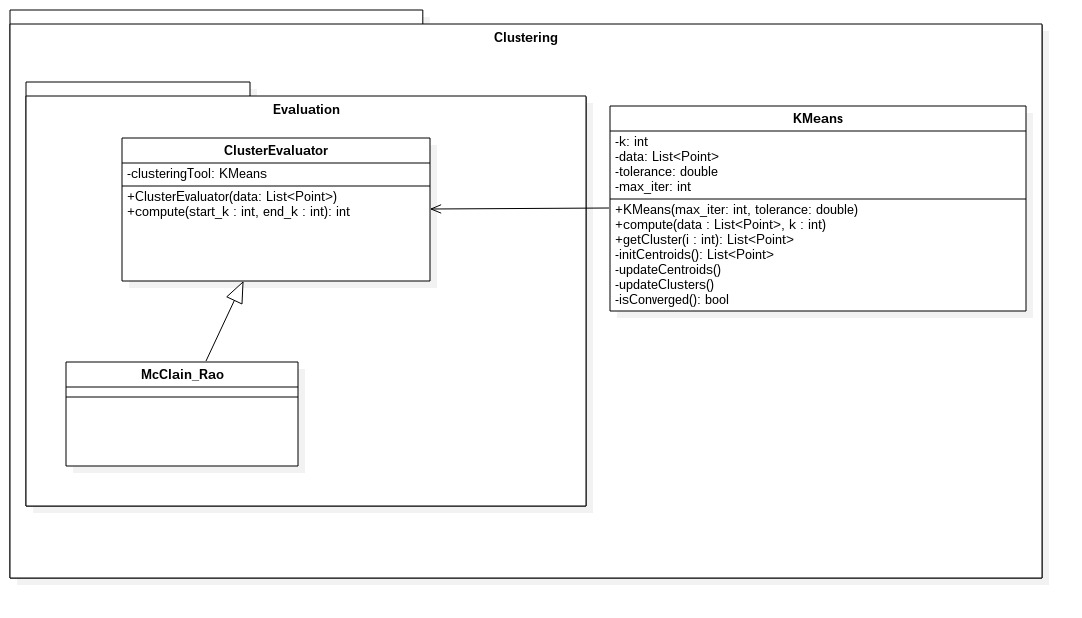
\includegraphics[width=0.8\textwidth]{images/clustering_class.jpg}
    \caption{Class diagrams of clustering module}
    \label{fig:clustering_class}
\end{figure}


%---------------------------------------------------------------
%---------------------------------------------------------------

\newpage
\subsection{Classification}

The classification module deals with the problems of classifying objects. Figure~\ref{fig:classification_class} shows the appropriate module. The \textit{Classifier} class contains a word generator. Note that the word generator itself, might correspond to real or synthetic data generation. The Classifier will then look for automaton which will classify these words in the best manner possible. The method of finding such automaton is the PSO algorithm. The \textit{PSO} class encapsulates the Particle Swarm Optimization algorithm. As arguments it takes the number of states and number of symbols in the alphabet, which will govern the swarm size and the dimensions of particles. Note that \textit{\_bestParticles} field is a list, since there can exist many best solution. Thus the \textit{getResults} shall return all such results and the Classifier class should be responsible for picking the most appropriate one.

Lastly the \textit{Particle} class simply encapsulates the particle used in PSO.

%
% CLASSIFICATION CLASS DIAGRAM
%
\begin{figure}[H]
	\centering
	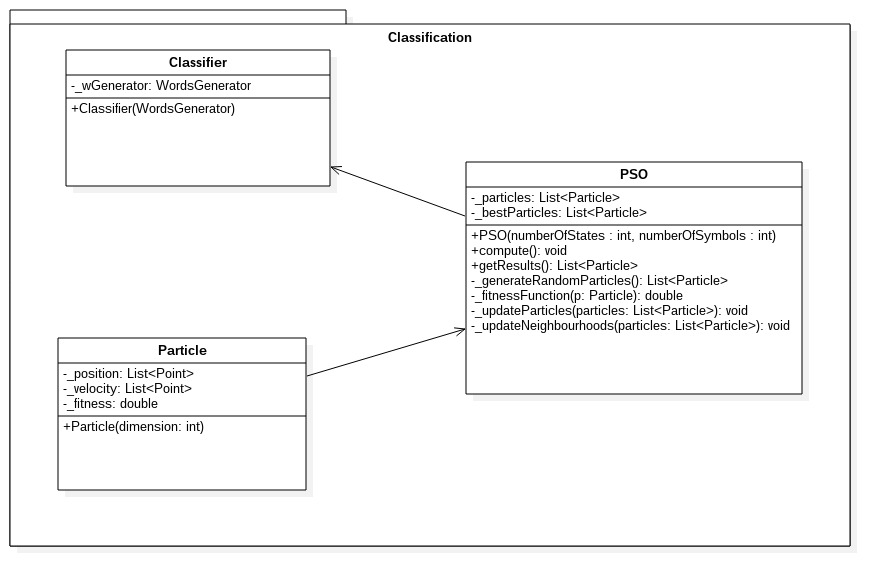
\includegraphics[width=0.8\textwidth]{images/classification_class.jpg}
    \caption{Class diagrams of classification module}
    \label{fig:classification_class}
\end{figure}



%---------------------------------------------------------------
%---------------------------------------------------------------
\newpage
\subsection{Utility}

The utility module is presented in figure~\ref{fig:utility_class}. \textit{Logger} class is responsible for printing and saving logs of the computations. It contains path to log directory and a path to specific file in which the logs should be saved. The one parameter method \textit{log}, prints the message to default file. The two parameter \textit{log} is used when the message should be saved in a different file.

The \textit{Console} class is responsible for loading flag parameters from the console, and updating the global settings. The global settings, containing all parameters of the computations are stored in \textit{Settings} class.

Finally a simple clock mechanism is proposed in \textit{Clock} class. The \textit{startClock} method starts measuring time until \textit{stopClock} is called which returns the time taken between both methods' calls. The time is encapsulated in \textit{TimeStamp} class.


%
% UTILITY CLASS DIAGRAM
%
\begin{figure}[H]
	\centering
	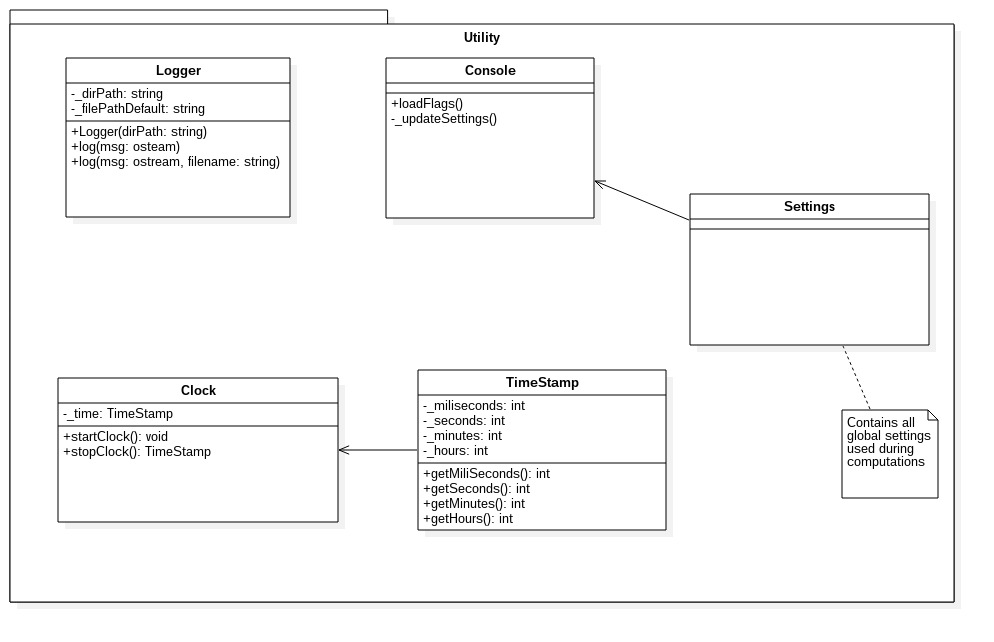
\includegraphics[width=0.8\textwidth]{images/utility_class.jpg}
    \caption{Class diagrams of utility module}
    \label{fig:utility_class}
\end{figure}


%---------------------------------------------------------------
%---------------------------------------------------------------
\newpage
\subsection{Math}

The math module shown in figure~\ref{fig:math_class} should contains all necessary classes from mathematical computations. The class \textit{Point} encapsulates a point in d dimensions. Such point can be instantiated with any type.

%
% MATH CLASS DIAGRAM
%
\begin{figure}[H]
	\centering
	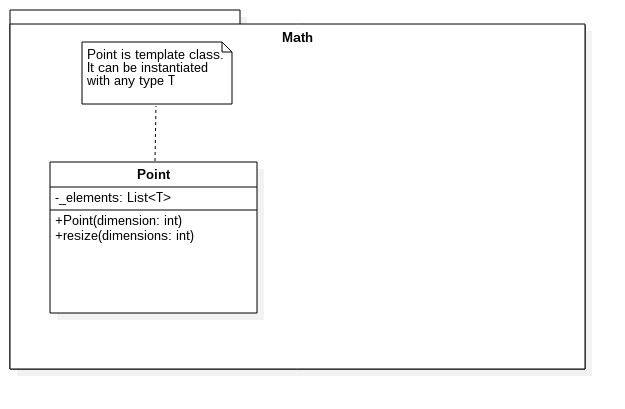
\includegraphics[width=0.8\textwidth]{images/math_class.jpg}
    \caption{Class diagrams of math module}
    \label{fig:math_class}
\end{figure}




%---- BD ----%

%
% DFA CLASS DIAGRAM
%
\newpage
\subsection{Deterministic Final Automaton}
In some sense this is most important class in the whole project. It represents automaton and its classical functionalities. Although class seems short, it uses objects of more sophisticated classes described in the subsections \ref{subsec:transition_table} and \ref{subsec:words_proc}. 

To start with we will describe fields of the class. \texttt{alphabet} is a vector of integers, which holds all symbols considered by automaton. It can be extracted from transition table using \texttt{\_acquireAlphabetFromTransitionTable()} method. Next and last one is \texttt{\_codedTransitionTable} object. In most general sense, object of this class mimics usage of transition table by allowing user to access and modify entries (see section \ref{sec:autom}), as well as coding and decoding table to form described in section \ref{sec:auto_dec}. 

Next we will look closer at constructors. First one generates random automaton based on provided number of states and alphabet. Alphabet takes values from interval [1,numberOfSymbols], hence it can be represented by single value: \texttt{numberOfSymbols}. Second constructor is suited to work with particle class. It reconstruct itself regarding to provided coded transition table, which in fact represents particle position. 

At the end a little bit about provided methods. \texttt{\_acquireAlphabetFromTransitionTable()} has been already mention - it loads alphabet from provided coded table. Rather auxiliary procedure. On the other hand, \texttt{checkRelationInducedByLanguage} is crucial for correct flow of the Particle Swarm Optimization. It takes two words and checks whether computations for each of them end up in the same state - if they are \texttt{true} value is return. Otherwise \texttt{false}. To perform this task \texttt{compute()} function is used. It takes word and returns number of state in which computations ended.

\begin{figure}[H]
	\centering
	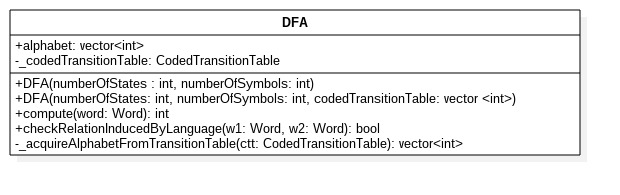
\includegraphics[width=0.9\textwidth]{images/dfa.jpg}
    \caption{Class diagram of Deterministic Finite Automaton}
    \label{fig:dfa_class}
\end{figure}

%
% WORD PROCESSING CLASS DIAGRAM
%
\newpage
\subsection{Words Processing}
To perform words generation/processing we will use classes presented on figure \ref{fig:words_processing_class}.

Since it happens to be largest and most important of all four, let us first focus on \texttt{WordsGenerator} class. Its main purpose is to create words using rules described in section \ref{section:Algorithms}. There are in fact two type of conditions to cover:
\begin{itemize}
\item parametrical, where the class checks global parameters related to word processing
\item hamming condition, generated word of some length, let us say $n$, must have hamming distance between all (up to now) generated words of length $n$ smaller than some defined constant (see \ref{section:Algorithms} for reference)
\end{itemize}

Check of the first one is done via \texttt{\_checkGlobalConsitions()} and latter one is covered by \texttt{\_hammingCondition()}. As one can easily see, \texttt{\_hammingDistance()} method is just an auxiliary procedure for work related to checking hamming condition. Although method \texttt{\_generateRandomWordOverAlphabet} speaks for itself, \texttt{\_generateRandomWordStartinWith} needs some explanation. As we are forced to firstly produce words starting with different symbols of alphabet (again section \ref{section:Algorithms}), this method provides a way to create such a word with hamming condition checked. User specifies only starting symbol and length of the word and procedure returns random word starting with particular symbol and of specified length. There are only two public methods: constructor, which forces user to specify alphabet and \texttt{getPairs()}. The last one's ability is to gather all generated words and combine them into pairs. Such approach is forced by PSO's fitness function. 

Despites its vague name, \texttt{BagOfWords} is class which preserves set of words in form of an unordered map, where keys are lengths and entries are vectors of words of specified length. It enables easy access to words of some particular length. We took such approach because most comparisions in the \texttt{WordsGenerator} class is done by checking hamming condition, which concerns words of the same length. What is more, section \ref{section:Algorithms} obliged us to create 3 disjunctive sets of words: $\Omega_S$, $\Omega_M$ and $\Omega_L$ and using this class we can fulfil this need, preserving all desired functionality. When needed one can always gather all words as a vector using \texttt{getAllWords()} method.

Last two classes were created to make code more transparent. \texttt{PairOfWords} simply wraps two words together and \texttt{Word} class supplies user with short set of methods operating on vector of integers (which simulates a word). As mentioned they are more needed because their names than actual functionalites.

\begin{figure}[H]
	\centering
	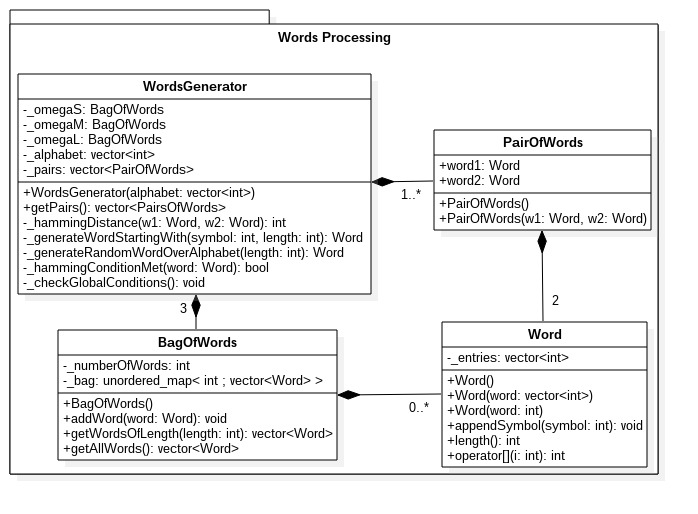
\includegraphics[width=0.8\textwidth]{images/words_processing.jpg}
    \caption{Class diagram of words processing clases.}
    \label{fig:words_processing_class}
\end{figure}

%
% TRANSITION TABLE CLASS DIAGRAM
%
\newpage
\subsection{Transition Table}
Classes used to model behaviour of transition table are presented on figure \ref{fig:trans_table_class}. 

\textcolor{red}{Remark:} It is worth to notice that in all consecutive classes, entries of transition tables stays as a vector of integers. Each table, beginning with \texttt{StandardTransitionTable}, provides its own way to read values from the vector either via overloading \texttt{operator ()} or by implementing methods.

As one can see, starting from most general \texttt{TransitionTable} and going up on chains of inheritance classes broad they abilities. Base class provides only methods for loading automaton from file specified via \texttt{url} string. It is able to either load it symbol by symbol ( \texttt{\_loadOneSymbol()} ) or fill up all entries at once - \texttt{\_loadEntries()}. Entries at this level can not be interpreted using any transition table type - it is just raw data.

Next, one can create \texttt{StandardTransitionTable}, which interprets \texttt{\_entries} as a table where columns represents symbols and rows are states. Classes, which will inherit from this one are provided with method \texttt{\_accessTransitionTable()} and for public usage \texttt{operator ()} has been overloaded. Both approaches force to pass symbol and state and as a results guarantee state. 

Thrid  is \texttt{PerSymbolTransitionTable}, which is more suited for computer interpretation of automaton. It assumes that each symbol has its own table. Each table's column and rows represents consecutive states and entries takes values equal to either $0$ or $1$. Such a values describe situation when "two states are not connected" and "there is connection between states", repsectively. Simmiraly to \texttt{StandardTransitionTable}, there are two ways to acces table. Public access is provided by overloaded \texttt{operator ()} and protected access is anabled via \texttt{\_isTransition()} method. Both needs two states and symbol to determine whether there is connection or not, hence return value is of boolean type.

Last but not least, we have \texttt{CodedTransitionTable} class. First observable difference appears in constructors - this class enables to initialize transition table either via loading and coding automaton from file or accepting coded automaton and decoding it to achieve transition table. Such approach has been forced by Particle Swarm Optimization algorithm. TO be a little bit more precise: paticles are represented by coded deterministic finite automata and need to be updated, which causes automata to change. In such a case we just create new automaton from updated particle's coded DFA table. \texttt{\_getCodedTransitionTable}, as name says, returns coded table, which then can be used as a position of particle within PSO space. All other methods concerns either coding or decoding procedures and are described more in section \ref{section:Algorithms}.




\begin{figure}[H]
	\centering
	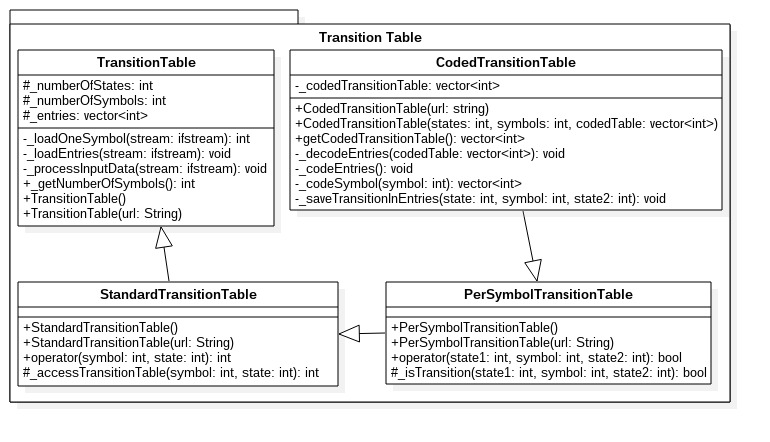
\includegraphics[width=0.9\textwidth]{images/transition_table.jpg}
    \caption{Class diagram of classes implementing different transition tables notations.}
    \label{fig:trans_table_class}
\end{figure}


%
% GUI CLASS DIAGRAM
%
\newpage
\subsection{Graphical User Interface}
\begin{wrapfigure}{c}{0.7\textwidth}
  \begin{center}
    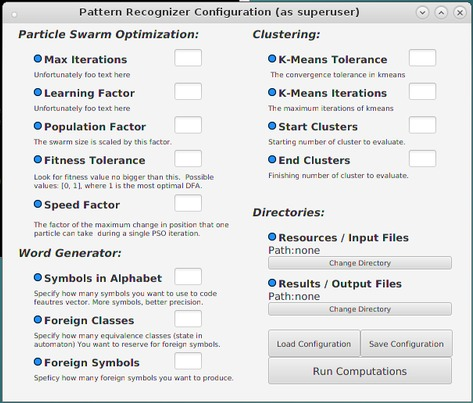
\includegraphics[width=0.7\textwidth]{images/mock_gui.jpg}
  \end{center}
  \caption{GUI Mockup}
  \label{fig:gui_look}
\end{wrapfigure}

Classes necessary to model and develop GUI are presented on figure \ref{fig:gui_classes}. On the other hand, look that we are trying to achieve is roughly sketch on figure \ref{fig:gui_look}.

As one could image, because of simplicity of the interface, there is nothing fancy in class diagram. \texttt{MainWindow} handles loading .fxml file and starting the application. On the oder hand, class \texttt{MainWindowControls} is in charge of events processing. It handles any event occurred regarding user interface objects and performs appropriate actions. Since main functionality of this part of the application is to set up global configurations, when some value within an user interface object will change, so will corresponding entry in configuration file. One can easily load and save configurations files, as well as changing directory of input and output files. Presented figure \ref{fig:gui_look}, depicting design of the application, is definitely not the final one and in future it might contain e.g. text labels with more informations about features or some loading bars. Main look of the program should be defined in .fxml, which will not be presented in this paper due to its irrelevancy and numerous way of implementations. 

\begin{figure}[H]
	\centering
	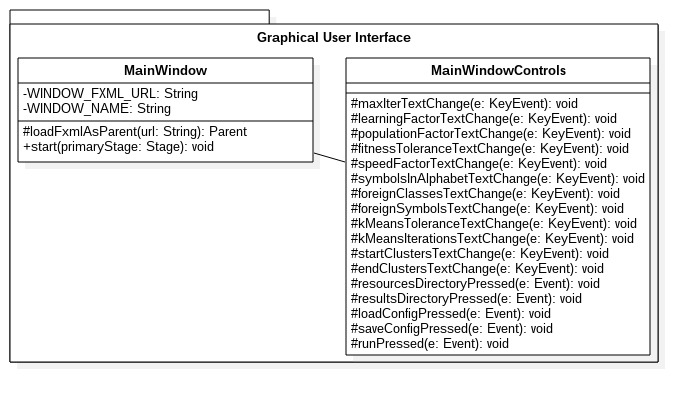
\includegraphics[width=0.9\textwidth]{images/gui.jpg}
    \caption{Class diagram of gui classes}
    \label{fig:gui_classes}
\end{figure}




\section{Bibliography}

\begin{thebibliography}{1}

\bibitem{javafx_description} \url{http://docs.oracle.com/javafx/2/overview/jfxpub-overview.htm}	


\bibitem{pso_origin} 
Eberhart, R. C. and Kennedy, J. A new optimizer using particle swarm theory. Proceedings of the sixth international symposium on micro machine and human science pp. 39-43. IEEE service center, Piscataway, NJ, Nagoya, Japan, 1995.

%\bibitem{pso_anal}
%Maurice Clerc. Stagnation analysis in particle swarm optimization or what happens when nothing happens, http://hal.archives-ouvertes.fr/hal-00122031. Technical report, 2006.



\bibitem{pso_bias} 
William M. Spears, Derek T. Green and Diana F. Spears. Biases in particle swarm optimization. International Journal of Swarm Intelligence Research, 1(2):34-57, 2010.




\bibitem{pso_11}
M. Clerc. (2011). Standard Particle Swarm Optimisation Available: http://hal.archives-ouvertes.fr/hal-00764996 

	
\end{thebibliography}



\end{document}


